% This is samplepaper.tex, a sample chapter demonstrating the
% LLNCS macro package for Springer Computer Science proceedings;
% Version 2.20 of 2017/10/04
%
\documentclass[runningheads]{llncs}
%
\usepackage{graphicx}
% Used for displaying a sample figure. If possible, figure files should
% be included in EPS format.
%
% If you use the hyperref package, please uncomment the following line
% to display URLs in blue roman font according to Springer's eBook style:
% \renewcommand\UrlFont{\color{blue}\rmfamily}

\begin{document}
%
\title{Fine Grain Lung Nodule Diagnosis Based on CT using 3-D Convolutional Neural Network}
%
%\titlerunning{Abbreviated paper title}
% If the paper title is too long for the running head, you can set
% an abbreviated paper title here
%
\author{
}
%
\authorrunning{}
\titlerunning{Fine Grain Lung Nodule Diagnosis}
% First names are abbreviated in the running head.
% If there are more than two authors, 'et al.' is used.
%
\institute{
}
%
\maketitle              % typeset the header of the contribution
%
\begin{abstract}
As the core step of lung nodule analysis, lung nodule diagnosis comprises two important tasks: False Positive Reduction (FPR) and Malignancy Suspiciousness Estimation (MSE). Many studies tackle these two tasks separately. However, these two tasks share a lot of similarities and have connections with each other, since MSE is the successive step of FPR, and both tasks can be deemed as the lung nodule labeling problems. In this paper, we split the label `real nodule' defined in FPR into two new finer grain labels, namely `low risk' and `high risk', which are defined in MSE. In such way, we merge these two separated issues into a unified fine grain lung nodule classification problem. Finally, a novel Attribute Sensitive Multi-Branch 3-D CNN (ASMB3DCNN) is proposed for performing the fine grain lung nodule classification. We evaluate our model on LIDC-IDRI and LUNA16 datasets. Experiments demonstrate that ASMB3DCNN can efficiently address the two tasks above in a joint way and achieve the promising performances in comparison with the state-of-the-arts.


\keywords{Joint Learning \and Lung Nodule Diagnosis \and Convolutional Neural Network \and Computed tomography (CT) \and Computer-aided detection and diagnosis (CAD)}
\end{abstract}

\section{Introduction}
Each year, there are 8.2 million deaths caused by cancer in the worldwide. Lung cancer accounts for the highest number of mortalities i.e. 1.59 million \cite{Wild2014International}. However, according to statistics, most patients diagnosed with lung cancer today already have advanced disease (40\% are stage IV, 30\% are stage III), and the current 5-year survival rate is only 16\% \cite{Bach2012Benefits}, which indicates that early diagnosis and treatment can effectively improve survival chance of lung cancer patients. As the core step of lung nodule analysis, classifying a large number of detected nodules by the radiologists, which includes False Positive Reduction (FPR) and Malignancy Suspiciousness Estimation (MSE), can be very time-consuming. Small nodules are very difficult to be found and can be confused with normal tissues. Long time reading work can also cause the fatigue of the radiologists and reduce the work efficiency. Thus, developing a fast, robust and accurate CAD system to perform automated diagnosis of lung nodules is meaningful and important\cite{Greenspan2016Guest}, many CAD systems have been designed to help the radiologists like \cite{rajpurkar2017chexnet} \cite{wang2018tienet} \cite{Causey2018Highly} \cite{nanwu2019dnn}.

\begin{figure}[*t]
\centerline{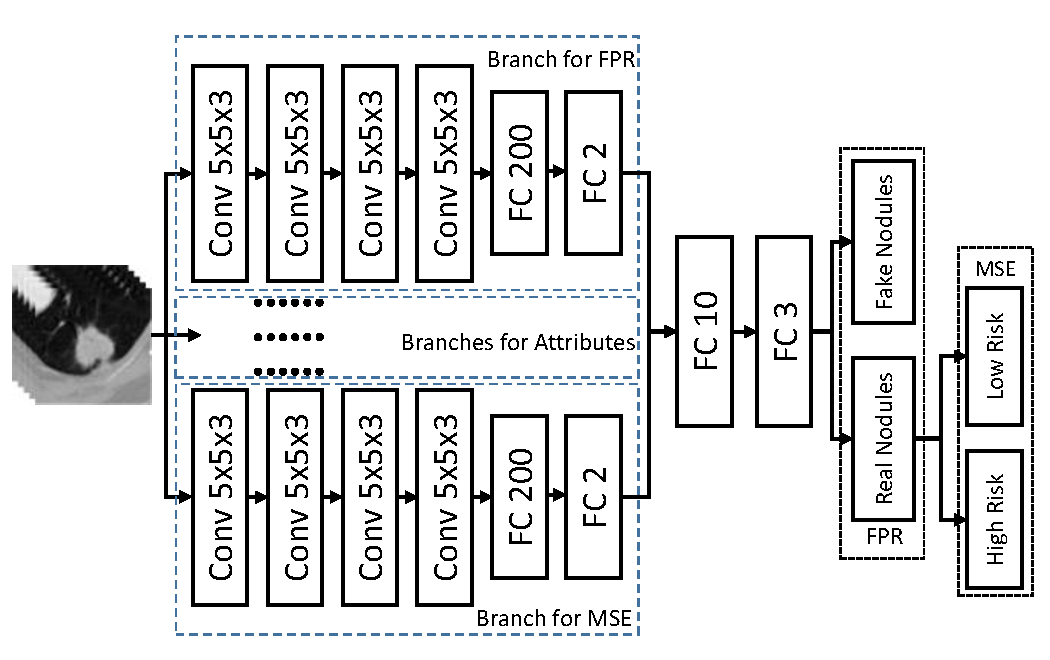
\includegraphics[width=100mm]{fig1.pdf}}
\vspace{-0.0cm}
\caption{Architecture of ASMB3DCNN}
\vspace{-0.5cm}
\label{fig1}
\end{figure}


To the best of our knowledge, most studies considered FPR and MSE as two totally separated problems.

In the task of FPR, Qi Dou et al. \cite{Qi2016Multilevel} designed a multilevel contextual 3-D Convolutional Neural Networks (3-D CNN) to encode richer spatial information and extract more discriminative representations via the hierarchical architecture trained with 3-D samples.

In the task of MSE, Wei Shen et al. \cite{Shen2017Multi} exploited CNN to differentiate lung nodules and proposed a Multi-crop CNN network structure. Sarfaraz Hussein \cite{Hussein2017Risk} used multi-task learning model based on 3-D CNN, which showed that information of high-level attributes can help to improve the performance of the model. Botong Wu\cite{Wu2018Joint} designed PN-SAMP, which can also provide related evidences and segmentation information to radiologists.
Study in \cite{shen2019interpretable} is very instructive, they  use the attributes information to predict the malignancy level. Their model HSCNN share weights between first two convolutional layers, then splits into a few branches to finish tasks of predicting attributes and  feeds predictions of attributes into  dense layers to predict malignancy level.
Jason Causey et al.\cite{Causey2018Highly} proposed NoduleX. In Nodulex, they leveraged a deep CNN (more than 10 CNN layers) to tackle FPR and MSE tasks separately, and they also proved that these two tasks are similar.

Extensive studies show that 3-D CNN is a powerful approach for addressing both MSE and FPR issues in a separated way \cite{Qi2016Multilevel}\cite{Causey2018Highly}\cite{Shen2015Multi}\cite{Kang20173D}, since it is deemed as the best choice for keeping 3-D spatial information in the CT scans \cite{Yorozu1987Electron}.


 As MSE is the successive step of FPR, the label `real nodule' defined in FPR can be further divided into two new finer grain labels, namely `low risk' and `high risk'. Moreover, these two tasks share lots of high-level attributes.According to the findings above, we intent to merge these two tasks into a unified fine grain lung nodule diagnosis problem and present a novel Attribute Sensitive Multi-Branch 3-D CNN (ASMB3-DCNN) to address this unified issue. In this model, we also analyse the sensitivity of attributes. Rather than use all attributes provided by dataset, we select specific attributes to improve the performance of model. 
The architecture of ASMB3DCNN is shown in Fig ~\ref{fig1}.


Our main contributions are in four-folds:

(1) We analyze backgrounds of False Positive Reduction (FPR) and  Malignancy Suspiciousness Estimation (MSE) tasks, and merge them into a unified task.

(2) We measure the sensitivities of attributes and select the most reliable attributes to yield an attribute sensitive version of 3-D CNN for fine grain lung nodule diagnosis.

(3) We design a method of normalization to capture different sizes of inputs according to the slices-thickness and pixel-spacing which has been empirically proved that such strategy can improve accuracy of classification and reduce the burden of calculation.

(4) Beyond FPR and MSE,we extend the proposed approach to predict nodule attributes,which could potentially assist radiologists in evaluating malignancy uncertainty.

The rest of paper is organized as follows: Section~\ref{method} introduces the methodology of our works; experiments are presented in section~\ref{exp}; the conclusion is finally summarized in section~\ref{conclude}.



\section{Method}
\label{method}
Since Malignancy Suspiciousness Estimation (MSE) is the successive task of False Positive Reduction (FPR) in the lung nodule diagnosis, MSE essentially performs a further classification on the positive samples labeled by FPR. In such way, we can further categorize the positive samples into two finer categories, namely `low risk' and `high risk', and these two tasks can be unified as a fine grain lung nodule classification issue. In this paper, we present a novel 3-D CNN named  Attribute Sensitive Multi-Branch 3-D CNN (ASMB3DCNN) to address such issue and then the tasks of FPR and MSE can be jointly tackled. 

We firstly analyse the sensitivity of all attributes and select attributes which are more sensitive to the malignancy level.  Then we use a normalization method to resize nodules in CT scans into the same scale and feed them into different branches to predict level of different attributes. The last step is to train all branches jointly to perform the unified fine grain lung nodule diagnosis classification.


\subsection{Sensitivity Analysis of Attributes}
\label{select}
The study in \cite{Hussein2017Risk} indicates that the attributes can facilitate the solution of MSE. However, not all attributes are sensitive to (or strongly correlated to) the level of malignancy suspiciousness of lung nodules. Thus, here we intend to analyse the sensitivities of attributes to malignancy suspiciousness level via measure the variance of the proportion of high risk lung nodules under different levels of attributes as follows:
\begin{equation}
\mathcal{S} = \frac{1}{n-1}\sum_{i=1}^n (X_i - \bar{X})^{2}
\end{equation}
where $n$ is the number of score levels,  $X_i$ is the proportion of malignant nodules, $\bar{X}$ is the average of proportion.

There are 8 attributes, namely `subtlety', `internalStructure', `calcification', `sphericity', `margin', `lobulation', `spiculation' and `texture'.
We measure the sensitivity of these attributes in training set of LIDC-IDRI dataset, rank them by their sensitivities and tabulate the results in Table~\ref{tab2}. We find the top 2 sensitive attributes are `internalStructure' and `calcification' whose sample distributions are extremely unbalanced as shown in Table~\ref{tab3}.  In category of `internalStructure', 99.8\% of nodules are in level 1 and 2. In category of `calcification', 99.8\% of nodules are in level 3,4,5 and 6. This makes us very hard to train the reliable predictors for these two attributes via using the training samples, and the unreliably predicted attributes may corrupt the performance of the lung nodule diagnosis system. Thus, we choose `subtlety', `lobulation', `spiculation' (their ranks are from 3 to 5) as complementary information for lung nodule classification. In order to prove that our selection of attributes can actually help the model, we also train the model with  `subtlety', `lobulation', `spiculation' ,`sphericity',`margin' and `texture',  and results shown in Table~\ref{tab4} prove that model with 3 selected attributes is better than model with 6 attributes.The architecture of each branch will be discussed later in section ~\ref{architecture}.
Examples of nodules with different level attributes are shown in Table~\ref{nodules}, nodules framed with red rectangles are high risk nodules. We can clearly see that nodules with high level attributes like `lobulation' are more likely to be malignant.

\begin{figure}[htb]
\centerline{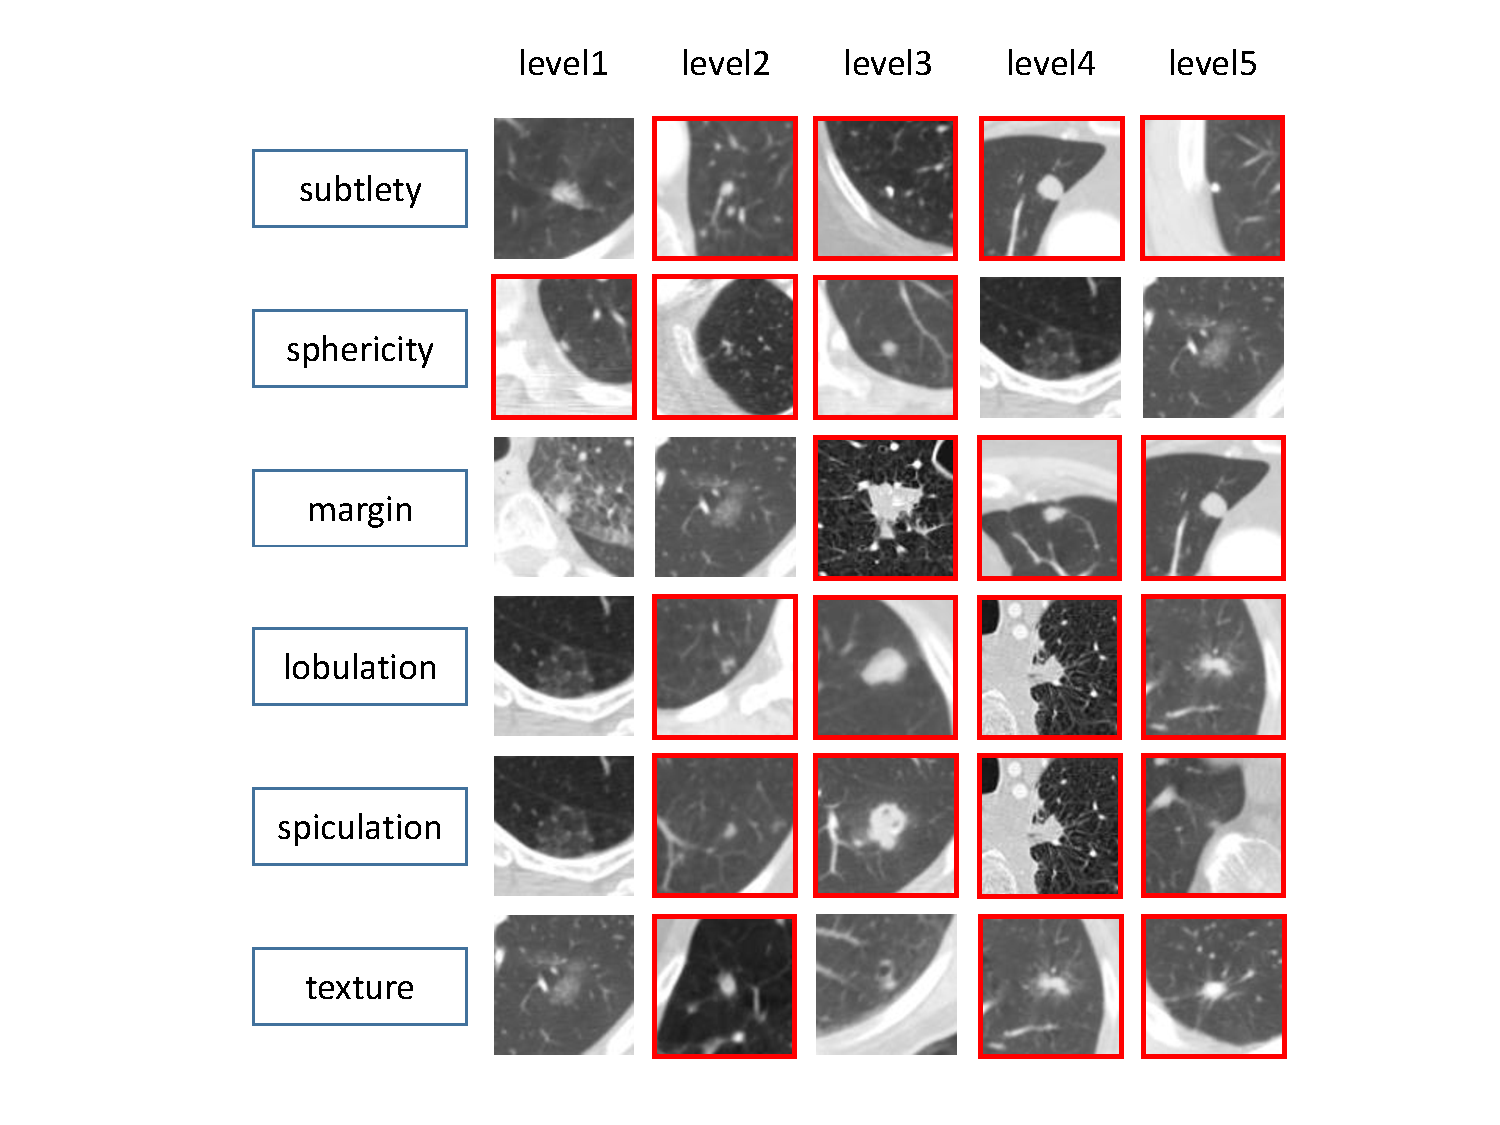
\includegraphics[width=125mm]{nodules.pdf}}
\vspace{-0.5cm}
\caption{Nodules with different level attributes(nodules framed with red rectangles are high risk nodules)}
\vspace{-0.5cm}
\label{nodules}
\end{figure}

\begin{table*}[htb]
\caption{Proportion of Malignant Nodules in Each Level}
\vspace{-0.5cm}
\begin{center}
\begin{tabular}{|c|c|c|c|c|c|c|c|c|}
\hline
\textbf{Attributes}&\multicolumn{6}{|c|}{\textbf{Attributes Rate}} & \textbf{Sensitivity}&\textbf{Attribute}\\
\cline{2-7}
\textbf{Category}& 1&2&3&4&5&6& \textbf{(Variance)}&\textbf{Rank} \\
\hline
subtlety& 2.56\% &5.92\% & 5.53\% & 17.23\% & 44.61\% & - & 0.030&5\\
internal-Structure& 18.90\% & 47.62\% & 50.00\% & 0.00\% & 0.00\% & - &0.060&1\\
calcification& 0.00\% &0.00\% & 0.00\% & 1.80\% & 10.81\% & 21.88\% & 0.057&2 \\
sphericity& 0.00\% & 17.28\% & 23.00\% & 20.79\% & 8.60\% & - &0.009&6\\
margin& 20.56\% & 23.83\% & 28.36\% & 21.80\% & 9.78\% & - &0.004&7\\
lobulation& 6.77\% & 26.67\% & 54.55\% & 56.12\% & 13.79\% & - &0.052&3\\
spiculation& 7.47\% & 31.39\% & 58.70\% & 57.39\% & 41.94\% & -&0.045& 4\\
texture& 11.56\% & 20.35\% & 20.86\% & 23.57\% & 18.41\% & - &0.002&8\\
\hline

\end{tabular}

\label{tab2}
\end{center}
\vspace{-0.5cm}
\end{table*}

\begin{table}[htb]
\caption{Number of  Nodules in Each Level}
\begin{center}
\begin{tabular}{|c|c|c|c|c|c|c|}
\hline
\textbf{Attributes}&\multicolumn{6}{|c|}{\textbf{Attributes Rate}} \\
\cline{2-7}
\textbf{Category}& 1&2&3&4&5&6\\
\hline
subtlety&117&321&506&1097&594&-\\
internal-Structure&2609&21&2&2&1&-\\
calcification&3&2&187&111&74&2258\\
sphericity&5&191&613&1419&407& -\\
margin& 107&277&342&1101&808& - \\
lobulation&1433&855&220&98&29& - \\
spiculation&1647&704&138&115&31& - \\
texture&173&113&139&488&1722& - \\
\hline
\end{tabular}
\vspace{-0.5cm}
\label{tab3}
\end{center}

\end{table}
%\vspace{-0.8cm}


\subsection{Normalization}
The slice-thickness ranges from 0.6 mm to 5.0 mm, the pixel-spacing ranges from 0.4609375 mm to 0.9765625 mm. Wei Shen et al. \cite{Shen2017Multi} normalized images using spline interpolation to have a fixed resolution with 0.5 mm/voxel along all three axes, all images will be re-sampled before cropping nodules, which is time-consuming. Moreover, coordinates of nodules will be affected during re-sampling.

To reduce the burden of computation, we adjust the input size according to slice-thickness and pixel-spacing and resize the input after cropping. The length, width and height of inputs are set to 30mm  $\footnote[1]{In clinical, nodules larger than 30mm in diameter are called lung masses and will not be discussed here}$. 
Fewer slices are needed if the slice-thickness gets larger.
The coordinates of nodules are not affected.
Then we resize the input into $20\times20\times10$ using spline interpolation since ASMB3DCNN needs a size-fixed input. Fig~\ref{normalization} shows that after normalization, the accuracy of six branches are improved in LIDC-IDRI dataset, accuracy of branch margin drops 1.09\%, and accuracy of FPR is still the same.

\begin{figure}[htb]
\centerline{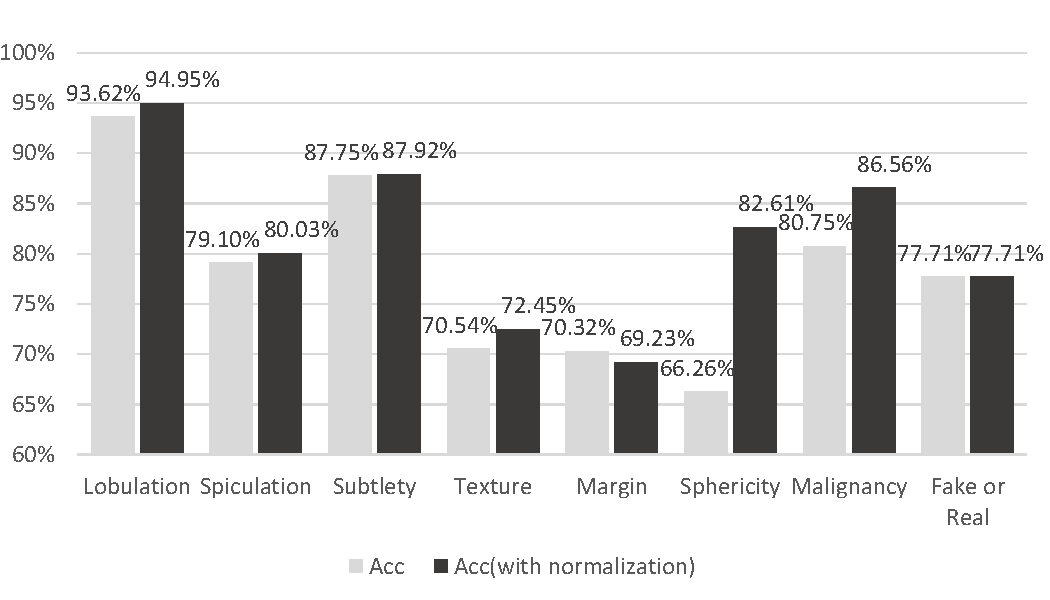
\includegraphics[width=80mm]{fig2.pdf}}
\vspace{-0.5cm}
\caption{Comparison of Accuracy After Normalization}
\vspace{-0.5cm}
\label{normalization}
\end{figure}






\subsection{Architecture of ASMB3DCNN}
\label{architecture}
There are eight branches in the proposed Attribute Sensitive Multi-Branch 3-D CNN(ASM3DCNN), follow the study ~\cite{nanwu2019dnn}, our model is split at the very first, and all branches share the same architecture as shown in Fig~\ref{fig1}.
Like model in~\cite{Qi2016Multilevel}, we use kernels with size of  ~$5\times5\times3$, ~$1\times1\times1$ and adjust the architecture according to the results of experiments. Each branch consists of four 3-D convolutional layers (the kernel sizes are $5\times5\times3$, ~$5\times5\times3$, ~$5\times5\times3$, ~$1\times1\times1$, and the number of kernels are 64, 128, 256, 256 respectively), two fully-connected layers, and one softmax layer for giving an initial binary prediction to a specific attribute or a category.Between CNN layers, we use ReLU as activation function. In these eight branches, there are two branches used for predicting false positive(FPR) and malignancy suspiciousness(MSE) of a lung nodule respectively, and the other six branches are used for predicting the selected attributes, which have been empirically verified to be helpful for lung nodule diagnosis~ \cite{Hussein2017Risk}. 
We select the attributes based on the sensitivity analysis of attributes.  We fuse the outputs of these branches via two fully-connected layers and present the final classification via a softmax layer.In the training phase, we adopt the pre-training + fine-tuning strategy to train our network. Branches are trained separately and then the branches are combined with the fusion layers to perform a fine-tuning. We have tried different kinds of combination:(1)ASMB3DCNN(MSE/FPR)  has only one branch for MSE or FPR;(2)ASMB3DCNN(MSE/FPR+6 Attributes) contains one branch for MSE/FPR and all 6 attributes;(3)ASMB3DCNN(MSE/FPR+3 Attributes)  contains one branch for MSE/FPR and 3 selected attributes;(4)ASMB3DCNN(ALL) contains branches for MSE, FPR and 3  attributes. (5)ASMB3DCNN(Attributes only) contains branches only for attributes. Why we try these different combination will be discussed latter in section~\ref{exp}.

\section{Experiments and Results}
\label{exp}
\subsection{Datasets}
The Lung Image Database Consortium Image Collection (LIDC-IDRI) \cite{Armato2010WE}, is a public-available dataset, consisting of 1010 patients with chest CT scans. This dataset provides 36378 nodules and 2635 of them are analyzed by four experienced radiologists. Because of the small number of data, we rotate nodules $90^{\circ}$, $180^{\circ}$, and $270^{\circ}$ within the transverse plane.

Lung Nodule Analysis 2016 (LUNA2016) \cite{Aaa2016Validation} is a challenge for lung nodules detection and FPR. Its dataset is built based on LIDC-IDRI, while it removes nodules which are less than 3mm in diameter and provides more than 700 thousand fake nodules for FPR. Since then, we train the branches of six attributes and MSE using LIDC-IDRI dataset while train the branch of FPR using LUNA2016 dataset (samples from LIDC-IDRI dataset + fake nodule samples).


\subsection{Nodule Attributes Prediction Results}
In branches of attribute predictions, we binarize the  levels of attributes. More specifically, we label the nodules with level equal to or higher than 3 as `high', and the ones with level lower than 3 as `low'. Therefore, each branch of attribute prediction can be considered as a naive binary classifier.
Fig~\ref{normalization} presents the classification performance for each of the attribute-branches. We achieved mean accuracy(with normalization) of 94.95\%, 80.03\%,87.92\%, 72.45\%, 69.23\%, 82.61\% for lobulation, spiculation, subtlety, texture, margin, sphericity, respectively. As mentioned in \cite{Hussein2017Risk},nodule attributes can facilitate the solution of MSE, so we combine predictions of attributes with MSE.  Moreover, we find that these attributes information can actually help to improve FPR, since real nodules trend to have more obvious features and fake nodules trend have less obvious features. Finally, we combine attributes branches with FPR and MSE to perform both tasks together.
Meanwhile, we provide attributes information for radiologists and it will assist radiologists in evaluating the nodule classification result.


\subsection{Malignancy Suspiciousness Estimation}
\label{MSE}
Following the study \cite{Shen2017Multi}\cite{Causey2018Highly}, we exclude the nodules whose average malignancy scores are equal to 3. We respectively label the nodules whose average malignancy scores higher than 3 as `high risk nodules' and  label the nodules whose average malignancy score lower than 3 as `low risk nodules'.

Table~\ref{tab4} shows the performances of different versions of ASMB3DCNN in comparison with the state-of-the-arts. ASMB3DCNN(MSE), which uses the MSE branches only, is actually degraded as an ordinary single steam 3-D CNN. It obtains 86.6\% in accuracy and 84.5\% in AUC score respectively, while ASMB3DCNN (MSE+3  Attributes)  obtains 11.2\% and 11.1\% gains in accuracy and AUC score, these observations verify that the high-level attributes can indeed bring a boost in the performance of MSE.

Compared to  ASMB3DCNN (MSE+3  Attributes) ,  ASMB3DCNN (MSE+6  Attributes) obtains 93.8\% in accuracy.As shown in Table~\ref{tab2}, attributes like texture, have a low  variance of the proportion, which means branches of these attributes cannot provide useful features and information for decision process of MSE and corrupts the performances of the model.
We also train ASMB3DCNN(Attributes only) , it obtains only 67.6\%  in accuracy, it verifies that branch of MSE learn something more complex than combination of attributes.

 ASMB3DCNN(ALL)  performs less worse than ASMB3DCNN (MSE+3 Attributes) but gets a similar performance to NoduleX. It is not hard to understand this phenomenon, since FPR performs a superclass labeling instead of a simple classification from the perspective of the MSE task.  More specifically, the category `real nodule' in FPR, which can be seen as a superclass, includes all two categories of MSE, namely `low risk' and `high risk'. In such way, the output of FPR branch actually has not offered any useful information for discriminating the `high risk' and the `low risk' data, and even corrupts the performances a little bit. 

Study in \cite{shen2019interpretable} is very instructive, they also use the attributes information to predict the malignancy level, but HSCNN obtains 84.2\% in accuracy. In order to explain this phenomenon, we examine  the feature maps of the second convolutional layer for different attributes and find that convolutional kernels pay attention to different part of nodules in different branches. As shown in Fig~\ref{attri}, `subtlety' pays more attention to the center of nodules, `lobulation' and `spiculation' pay more attention to the edge of nodules, and `malignancy' pay attention to the whole view. Feature maps are conflict between attributes, so joint learning at first two convolutional layers may lead to interaction between branches and reduce the accuracy.


\begin{table*}[htb]
\vspace{-0.5cm}
\caption{Comparison with Other Studies for MSE}
\begin{center}
\begin{tabular}{|c|c|c|c|c|}
\hline

\textbf{\textit{Methods}}& \textbf{\textit{Accuracy}}& \textbf{\textit{Sensitivity}} & \textbf{\textit{Specificity}} & \textbf{\textit{AUC Score}} \\
\hline
ASMB3DCNN(ALL) & 0.961 & 0.900 & 0.991& 0.965\\
ASMB3DCNN(MSE+6 Attributes) &  0.938 &  0.845 & 0.979&  0.942\\
ASMB3DCNN(MSE+3 Attributes) & {\bfseries 0.978} & {\bfseries 0.957} & 0.993& {\bfseries 0.976}\\
ASMB3DCNN(MSE) & 0.866 & 0.696 & {\bfseries 0.999}& 0.845\\
ASMB3DCNN(Attributes only) & 0.676 & 0.395 &  0.798& 0.602\\
NoduleX\cite{Causey2018Highly}& 0.932 & 0.879 & 0.985 & 0.971 \\
Fuse-TSD\cite{Xie2017Fusing}&0.895&0.842&0.920&0.966 \\
MC-CNN\cite{Shen2017Multi}&0.871&0.77& 0.93&0.93\\
HSCNN\cite{shen2019interpretable}&0.842&0.705& 0.889&0.856\\
\hline
\end{tabular}
\label{tab4}
\vspace{-1cm}
\end{center}
\end{table*}


\begin{figure}[htb]
\centerline{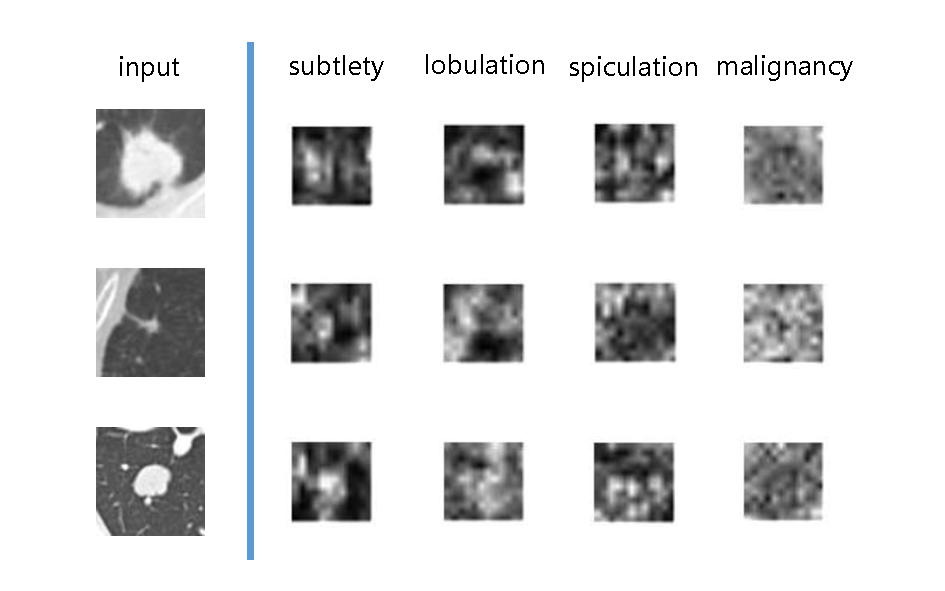
\includegraphics[width=100mm]{attri.pdf}}
\vspace{-0.5cm}
\caption{Feature Maps of Convolutional Layers for Different Attributes}
\label{attri}
\vspace{-0.5cm}
\end{figure}

\subsection{False Positive Reduction}
\label{FPR}
We conduct experiments via following the same experimental settings for nodule labeling in section~\ref{MSE}. As Table~\ref{tab5} shows,      ASMB3DCNN(FPR) obtains 77.7\% in accuracy and 75.3\% in AUC score respectively, while the ones of ASMB3DCNN (FPR+3 Attributes) are 96.9\% and 96.9\%, which shows the significant improvement over ASMB3DCNN (FPR). This phenomenon also indicates that the high-level attributes can benefit the solution of FPR problem. Another interesting observation is that ASMB3DCNN(ALL) outperforms ASMB3DCNN(FPR+3 Attributes) particularly in accuracy and sensitivity. The gains of ASMB3DCNN(ALL) over the FPR+Attributes version are 0.5\% and 3.7\% respectively. This verifies that the labels in a finer grain level is helpful to the solution of a classification task in a coarse level of labels. It also confirms the reasonability of our idea that these two separated issues can be merged into a unified fine grain lung nodule classification problem for better solving them together. Moreover, our proposed approaches have higher accuracy and specificity than other compared approaches. Although our approaches get slightly lower scores in comparison with NoduleX in sensitivity and AUC, NoduleX suffers from a heavier computation burden due to its deeper architecture. NoduleX has more than ten convolutional layers and max-pooling layers, while our models have only 4 convolutional layers.


\begin{table*}[htb]
\vspace{-0.5cm}
\caption{Comparison with Other Studies for FPR}
\begin{center}
\begin{tabular}{|c|c|c|c|c|}
\hline
\textbf{\textit{Methods}} & \textbf{\textit{Accuracy}} & \textbf{\textit{Sensitivity}}& \textbf{\textit{Specificity}} & \textbf{\textit{AUC Score}} \\
\hline
ASMB3DCNN(ALL)  & {\bfseries 0.974} & 0.935 &0.992 & 0.967 \\
ASMB3DCNN(FPR+3 Attributes)  &0.969 & 0.898 & 0.996 &0.969 \\
ASMB3DCNN(FPR) &0.777  & 0.697 & {\bfseries 0.997} &0.753 \\
Multilevel 3D-CNN\cite{Qi2016Multilevel} &- & 0.827 &-&-\\
UACNN(ccanoespinosa) &- &0.824 &-&- \\
NoduleX(CNN47+RF)\cite{Causey2018Highly} &0.946 & {\bfseries 0.948} & 0.943 & {\bfseries 0.984} \\
\hline

\end{tabular}
\label{tab5}
\vspace{-1cm}
\end{center}
\vspace{-0.5cm}
\end{table*}



\subsection{Fine Grain Lung Nodule Diagnosis}
We conduct experiments via extracting 7000 `fake nodules' from LUNA2016 and `real nodules' from LIDC-IDRI as the dataset(1:1 fake nodules to real nodules).
As Table~\ref{tab6} shows, the fine grain ASMB3DCNN(ALL) obtains 95.7\% in the accuracy of classifying Fake Nodules (FN), while the accuracy of ASMB3DCNN (ALL) in section~\ref{FPR} is 99.2\%. This is because the FPR branch is not trained with the `real nodule' in LIDC-IDRI, thus this branch has difficulty in classifying `low risk nodule' and `fake nodule', which has side effects on system.
On the other hand, ASMB3DCNN (ALL) in section~\ref{MSE} obtains 99.1\% in the accuracy of classifying Low Risk Nodules(LR) and 99.0\% in the accuracy of classifying High Risk nodules (HR), while the fine grain ASMB3DCNN(ALL) improve 0.5\% and 2.3\% in accuracy of classifying LR and HR respectively over ASMB3DCNN (ALL) in MSE,which means the FPR can help to make a distinction between `low risk nodules' and `high rick nodules'.
In general,the results confirm our idea about FPR and MSE are actually similar tasks and these two separated issues can be merged into a unified fine grain lung nodule classification problem .

\begin{table}[htb]
\vspace{-0.5cm}
\caption{Results of ASMB3DCNN(ALL)}
\vspace{-0.5cm}
\begin{center}
\begin{tabular}{|c|c|c|c|c|}
\hline
\textbf{\textit{Method}}& \textbf{\textit{Acc of FN}}& \textbf{\textit{Acc of LR}}& \textbf{\textit{Acc of HR}}  \\
\hline
Fine Grain & 0.957 & 0.996 & 0.923\\
MSE  & 0.992 & - & -\\
FPR & - & 0.991 &0.900 \\
\hline
\end{tabular}
\vspace{-0.5cm}
\label{tab6}
\end{center}
\vspace{-0.5cm}
\end{table}


\section{Conclusions}
\label{conclude}
In this paper, we propose ASMB3DCNN which can merge two tasks: False Positive Reduction (FPR) and Malignancy Suspiciousness Estimation (MSE) into a unified task: fine grain lung nodule diagnosis. Label `real nodule' defined in FPR can be split into two new finer grain labels, namely `low risk' and `high risk' defined in MSE.
We analyse the sensitivity of attributes and choose three attributes to improve the performance of the model.
Moreover, we design a method of normalization to improve the performance of each branch and reduce the burden of computation.
Experiments show that our model can achieve promising results in FPR, MSE and the task of fine grain lung nodule diagnosis,what's more,our method provides nodule attributes prediction to assist radiologists in evaluating malignancy uncertainty.

 We find that this classification system for nodules (1-6 levels and 8 attributes) is problematic. For extremely unbalanced attributes, we should adjust different evaluation criterion. Since attributes have conflict information,  sharing high level semantic information may bring negative effects to CNN models. 
Because of the strong learning ability of CNN and small number of dataset, all models for nodules classification have a risk of over-fitting. Moreover, few models use information of patients like smoking history and family history, which is different from diagnosis process in clinical. Our future work will also focus on fusing information of patients with CNN models to improve ability of generalization, and overcome the problems of predicting unbalance attributes.
 

%
% The following two commands are all you need in the
% initial runs of your .tex file to
% produce the bibliography for the citations in your paper.
\bibliographystyle{unsrt}
\bibliography{sigproc}  % sigproc.bib is the name of the Bibliography in this case
% You must have a proper ".bib" file
%  and remember to run:
% latex bibtex latex latex
% to resolve all references
%
% ACM needs 'a single self-contained file'!
%

\end{document}
